% 
% Permission is granted to copy, distribute and/or modify this document
% under the terms of the GNU Free Documentation License, Version 1.2
% or any later version published by the Free Software Foundation;
% with no Invariant Sections, no Front-Cover Texts, and no Back-Cover
% Texts.  A copy of the license is included in the section entitled "GNU
% Free Documentation License".




%%%%%%%%%%%%%%%%%%%%%%%%%%%%%%%%%%%%%%%%%%%%%%%%%%%%%%%%%%%%%%%%%%%%%%%%%%%%%%%%%%%%%%%%%% 
\section{Examples Guide}

We present here an example of an uncertainty propagation study based on a representation of the uncertainty thanks to a normal process $X(t)$. We define the input normal process using a spectral model, then we sample this model and propagate it through a linear model $L(x)$. Then, we recover the spectral model of the output process $Y(t)$ based on the output sample. This study is FFT intensive, and all the computations will be done using the FFTW object.

The input process is of dimension 1, and based on a normalized Cauchy spectral model defined by a spectral density $S(f)$ such that:
$$
  \forall f\in\Rset,\quad S_X(f)=\frac{2}{1+(2\pi f)^2}
$$

The linear model $L(x)$ is simply a scaling transformation:
$$
  \forall x\in\Rset,\quad L(x)=\alpha x
$$

The theoretical output process $Y(t)$ is also normal, stationnary and its spectral density is given by:
$$
  \forall f\in\Rset,\quad S_Y(f)=\frac{2}{1+(2\pi f)^2}
$$

A graphical comparison between this theoretical spectral density and the reconstructed one is given on figure \ref{DSPComparison}.

\begin{figure}[h]
  \centering
  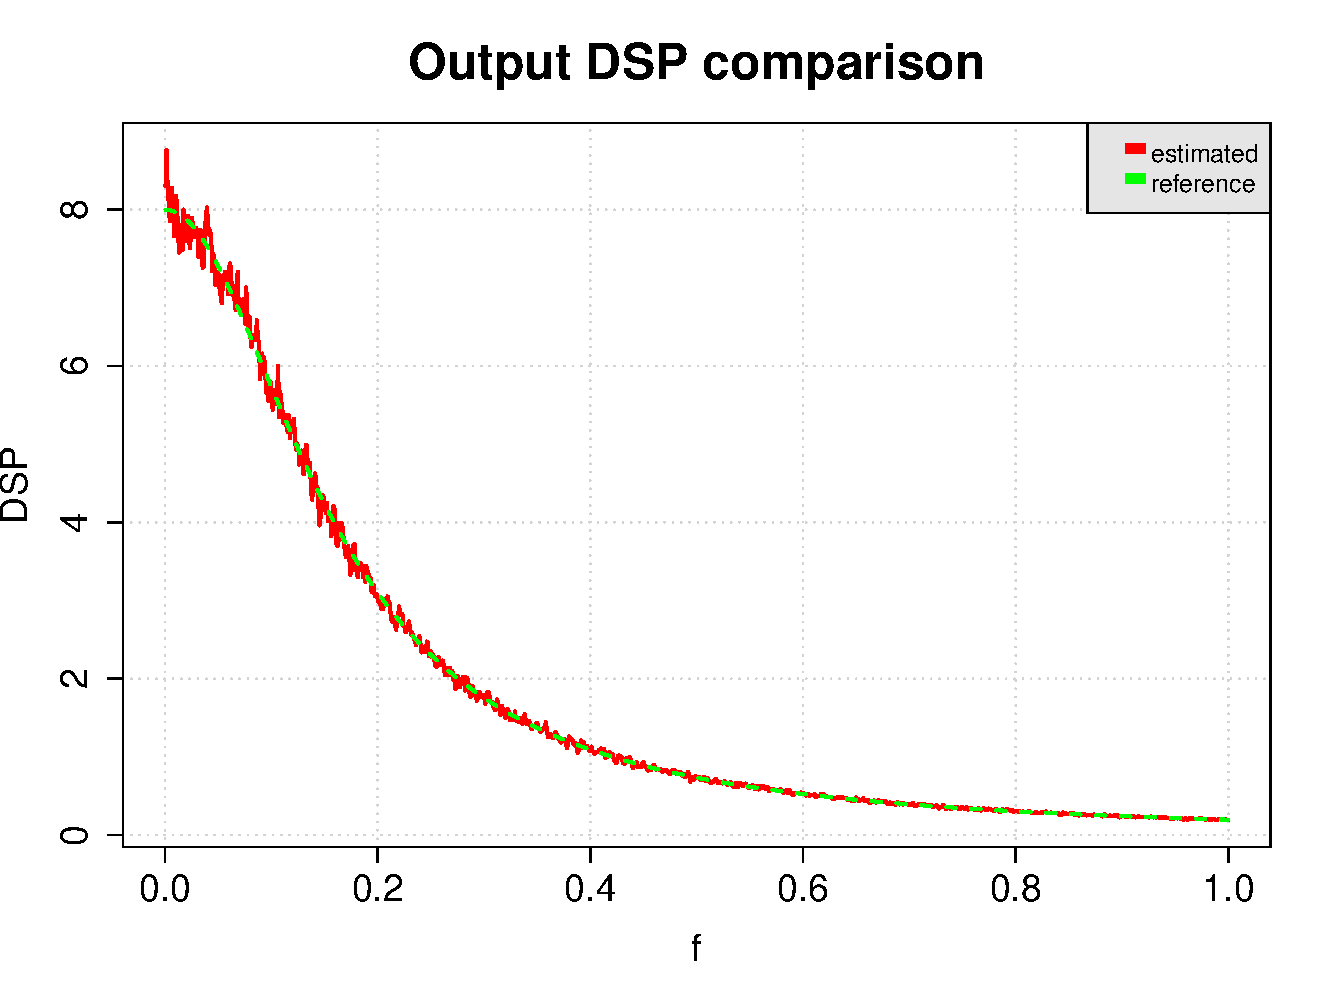
\includegraphics[width=\textwidth]{DSPComparison.pdf}
  \caption{Estimated spectral density (red) and theoretical one (green) of the output process}
  \label{DSPComparison}
\end{figure}

The speed-up with respect to the default OpenTURNS FFT algorithm is:
\begin{itemize}
\item a sampling time divided by a factor of 1.14
\item an estimation time divided by a factor of 2.31
\end{itemize}

on an Intel QuadCore Q9300 at 2.53GHz based laptop running Linux Mandriva 2010.2

\subsection{Python script}

\lstinputlisting[language=Python]{fftw_DSPEstimation.py}
